\documentclass[UTF8]{ctexbeamer}

\usepackage[europeanresistors,americaninductors,americanvoltages,americancurrents,siunitx]{circuitikz}
\usetikzlibrary{datavisualization}
\usetikzlibrary{datavisualization.formats.functions}
\usepgflibrary{arrows.meta}
\usepackage{pgfmath}
\usetikzlibrary{shapes.geometric,shadows,shapes.symbols}
%\pgfplotsset{compat=1.15}
\usefonttheme{serif}
\beamerdefaultoverlayspecification{<+->}      %环境会自动逐段显示

\begin{document}
\begin{frame}{中文演示文档}{An example}
 \begin{enumerate}
  \item 你需要将所有源文件保存为UTF-8 编码
  \item 你可以使用XeLaTeX、LuaLaTeX 或upLaTeX 编译
  \item 也可以使用(pdf)LaTeX 编译
  \item 推荐使用XeLaTeX 或LuaLaTeX 编译
 \end{enumerate}
\end{frame}

\begin{frame}[t]{方框图}
	\noindent\footnotesize
	\begin{tikzpicture}
        [auto,
        block/.style ={rectangle,draw,thick},
		block'/.style ={rectangle},
		input/.style ={draw=red,thick,ellipse,fill=red!20}]
		
		\newcommand\ORGX {0}
		\newcommand\ORGY {0}
		\newcommand\DX 	{3}
		\newcommand\DY  {1}

		\node [block] 	(A) at (\ORGX,\ORGY) {系统物理模型};\pause
		\node [block] 	(B) at (\ORGX,\ORGY-\DY) {系统方程};
		\path[draw,thick,-latex'] (A) -- (B);\pause

		\node [block] 	(C) at (\ORGX,\ORGY-2*\DY) {转移算子$H(p)$};
		\path[draw,thick,-latex'] (B) -- (C);\pause

		\node [input] 	(D) at (\ORGX+\DX,\ORGY-0.5*\DY) {初始状态};
		\node [block] 	(E) at (\ORGX+\DX,\ORGY-2*\DY) {零输入响应$r_{zi}(t)$};
		\path[draw,thick,-latex'] (C) --(E);
		\path[draw,thick,-latex'] (D)--(E);\pause

		\node [block] 	(F) at (\ORGX,\ORGY-3*\DY) {冲激响应$h(t)$};
		\path[draw,thick,-latex'] (C)--(F);\pause

		\node [block] 	(G) at (\ORGX-1.5*\DX,\ORGY-3*\DY) {单位阶跃响应$r_{\varepsilon}(t)$};
		\path[draw,thick,-latex'] (F)--(G);\pause

		\node [input] 	(H) at (\ORGX-0.7*\DX,\ORGY-\DY) {激励$e(t)$};
		\node [block] 	(I) at (\ORGX-1.5*\DX,\ORGY-4*\DY) {杜阿美尔积分};
		\path[draw,thick,-latex'] (H)|-(I);
		\path[draw,thick,-latex'] (G)--(I);\pause

		\node [block] 	(J) at (\ORGX,\ORGY-4*\DY) {卷积积分};
		\path[draw,thick,-latex'] (F)--(J);
		\path[draw,thick,-latex'] (H)|-(J);\pause
		
		\node [block] 	(K) at (\ORGX,\ORGY-5*\DY) {零状态响应$r_{zs}(t)$};
		\path[draw,thick,-latex'] (I)|-(K);
		\path[draw,thick,-latex'] (J)--(K);\pause

		\node [block] 	(L) at (\ORGX,\ORGY-6*\DY) {全响应$r(t)$};
		\path[draw,thick,-latex'] (K)--(L);
		\path[draw,thick,-latex'] (E)|-(L);

		\node [block'] 	(M) at (\ORGX,\ORGY-7*\DY) {$r(t)=r_{zi}(t)+r_{zs}(t)$};
		\path[draw,thick,-latex'] (L)--(M);
		
		
    \end{tikzpicture}    
\end{frame}
\section{1.1方框图2}
\begin{frame}[fragile]{方框图2}
	\begin{tikzpicture}
        [auto,
        decision/.style={diamond, draw=blue, thick, fill=blue!20,
        text width=5em,
        align=flush center,
        inner sep=1pt},
        block/.style ={rectangle, draw=blue, thick, fill=blue!20,
        %text width=5em,align=center, 
		rounded corners,
        %minimum height=4em
        },
        line/.style ={draw, thick,-latex',shorten >=2pt},
        cloud/.style ={draw=red, thick, ellipse,fill=red!20,
        minimum height=2em}]
        \matrix [column sep=10mm,row sep=3mm]
            {
                % row 1
                \node [cloud] (expert) {expert}; &
                \node [block] (init) {initialize model}; &
                \node [cloud] (system) {system}; \\
                % row 2
                & \node [block] (identify) {identify candidate model}; & \\
                % row 3
                \node [block] (update) {update model}; &
                \node [block] (evaluate) {evaluate candidate models}; & \\
                % row 4
                & \node [decision] (decide) {is best candidate}; & \\
                % row 5
                & \node [block] (stop) {stop}; & \\
        };
		\pause
        \begin{scope}[every path/.style=line]
            \path (init) -- (identify); \pause
            \path (identify) -- (evaluate);\pause
            \path (evaluate) -- (decide);
            \path (update) |- (identify);
            \path (decide) -| node [near start] {yes} (update);
            \path (decide) -- node [midway] {no} (stop);
            \path [dashed] (expert) -- (init);
            \path [dashed] (system) -- (init);
            \path [dashed] (system) |- (evaluate);
        \end{scope}
    \end{tikzpicture}
\end{frame}



\begin{frame}{列表环境}
	\begin{enumerate}
		\setcounter{enumi}{4}
		\item 离散谱,谱线间隔
		\item 离散谱,谱线间隔
	\end{enumerate}

	\begin{enumerate}[$(a)$]
		\item 离散谱,谱线间隔
		\item 离散谱,谱线间隔
	\end{enumerate}

	\begin{itemize}
		\item
			Shown from first slide on.
			\pause
		\item
			Shown from second slide on.
		\begin{itemize}
			\item
				Shown from second slide on.
				\pause
			\item
				Shown from third slide on.
		\end{itemize}
		\item
			Shown from third slide on.
			\pause
		\item
			Shown from fourth slide on.
	\end{itemize}
	Shown from fourth slide on.
	\begin{itemize}
		\onslide
		\item
			Shown from first slide on.
			\pause
		\item
			Shown from fifth slide on.
	\end{itemize}
\end{frame}

\frame{
\frametitle{作图}
\begin{tikzpicture}[scale=1]
					
					\draw [semithick][->] (-0.25,0) -- (3,0) node[right] {$t$};
					\draw [semithick][->] (0,-0.25) -- (0,1.5) node[right] {$\varepsilon(t)$} ;
					\draw [thin](0,1) -- (2.5,1);
					\draw (0,-0.25) node[left] {0} (0,1) node[left] {1};
\end{tikzpicture}

\[i(t) = \frac{2}{3}({e^{ - 0.5t}} - {e^{ - 2t}} )\]\\

			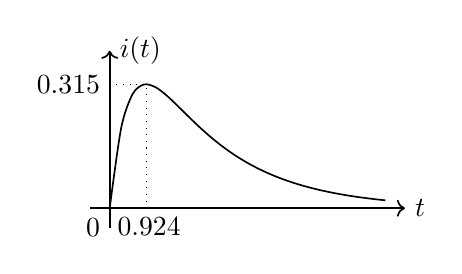
\begin{tikzpicture}[scale=0.5]
					\draw [semithick][->] (-0.5,0) -- (7.5,0) node[right] {$t$};
					\draw [semithick][->] (0,-0.5) -- (0,4) node[right] {$i(t)$} ;
					\draw (0,-0.5) node[left] {0} (0,3.15) node[left] {0.315}
								(1,0) node[below] {0.924};
					\draw [dotted] (0,3.15) -- (0.924,3.15) -- (0.924,0);
		 			
					\newcommand\SIGMA{6.66}
					%\datavisualization [school book axes, visualize as smooth line,x axis={label=$t$},y axis={label=$i(t)~A$}]
		      \datavisualization [xy Cartesian, visualize as smooth line]
					data [format=function] {
					var x : interval [0:7];
			    func y = \SIGMA*(exp(-0.5*\value x)-exp(-2*\value x));};
			\end{tikzpicture}	
}

\frame{
\frametitle{作图1}
单位冲激函数$\delta (t)$\\

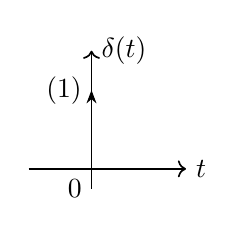
\begin{tikzpicture}[scale=1]
					
					\draw [semithick][->] (-0.8,0) -- (1.2,0) node[right] {$t$};
					\draw [semithick][->] (0,-0.25) -- (0,1.5) node[right] {$\delta(t)$} ;
					\draw [thin][-Stealth] (0,0)--(0,1);
					\draw (0,-0.25) node[left] {0} (0,1) node[left] {$(1)$};
\end{tikzpicture}

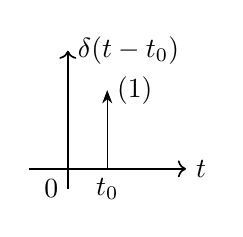
\begin{tikzpicture}[scale=1]
					
					\draw [semithick][->] (-0.5,0) -- (1.5,0) node[right] {$t$};
					\draw [semithick][->] (0,-0.25) -- (0,1.5) node[right] {$\delta(t-t_0)$} ;
					\draw [thin][-Stealth] (0.5,0)--(0.5,1);
					\draw (0,-0.25) node[left] {0} (0.5,1) node[right] {$(1)$} (0.5,0) node[below] {$t_0$} ;
\end{tikzpicture}					
}

\frame{
	\frametitle{作图2}
	\begin{circuitikz} 
 		\draw[semithick]	(0,0) to [L=1<\henry>](2.5,0) to [L=2<\henry>](5,0)
 			to	[R=1<\ohm>] (5,-2.5) to (5,-2.5)--(0,-2.5);
 		\draw[semithick]	(0,0) to 	[R,l_=1<\ohm>] (0,-1.5) to [V_=$e(t)$](0,-2.5);
    	\draw[semithick]	(2.5,0) to 	[C, l=1<\farad>,*-*] (2.5,-2.5)	;
    	\draw[semithick] [->] (1.25,-0.5) to [bend left=65,edge label'=$i_1(t)$] (1.25,-2);
    	 \draw[semithick] [->] (3.5,-0.5) to [bend left=65,edge label=$i_2(t)$] (3.5,-2);
 	\end{circuitikz}
}

	\begin{frame}[fragile]
	 	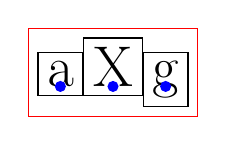
\begin{tikzpicture}
       		[every node/.style={draw=black,anchor=base,font=\huge}]
       	 		\matrix [draw=red]
        	{
            \node {a}; \fill[blue] (0,0) circle (2pt); &
            \node {X}; \fill[blue] (0,0) circle (2pt); &
            \node {g}; \fill[blue] (0,0) circle (2pt); \\
        	};
    	\end{tikzpicture}
	\end{frame}
\end{document}